\documentclass[1p]{elsarticle_modified}
%\bibliographystyle{elsarticle-num}

%\usepackage[colorlinks]{hyperref}
%\usepackage{abbrmath_seonhwa} %\Abb, \Ascr, \Acal ,\Abf, \Afrak
\usepackage{amsfonts}
\usepackage{amssymb}
\usepackage{amsmath}
\usepackage{amsthm}
\usepackage{scalefnt}
\usepackage{amsbsy}
\usepackage{kotex}
\usepackage{caption}
\usepackage{subfig}
\usepackage{color}
\usepackage{graphicx}
\usepackage{xcolor} %% white, black, red, green, blue, cyan, magenta, yellow
\usepackage{float}
\usepackage{setspace}
\usepackage{hyperref}

\usepackage{tikz}
\usetikzlibrary{arrows}

\usepackage{multirow}
\usepackage{array} % fixed length table
\usepackage{hhline}

%%%%%%%%%%%%%%%%%%%%%
\makeatletter
\renewcommand*\env@matrix[1][\arraystretch]{%
	\edef\arraystretch{#1}%
	\hskip -\arraycolsep
	\let\@ifnextchar\new@ifnextchar
	\array{*\c@MaxMatrixCols c}}
\makeatother %https://tex.stackexchange.com/questions/14071/how-can-i-increase-the-line-spacing-in-a-matrix
%%%%%%%%%%%%%%%

\usepackage[normalem]{ulem}

\newcommand{\msout}[1]{\ifmmode\text{\sout{\ensuremath{#1}}}\else\sout{#1}\fi}
%SOURCE: \msout is \stkout macro in https://tex.stackexchange.com/questions/20609/strikeout-in-math-mode

\newcommand{\cancel}[1]{
	\ifmmode
	{\color{red}\msout{#1}}
	\else
	{\color{red}\sout{#1}}
	\fi
}

\newcommand{\add}[1]{
	{\color{blue}\uwave{#1}}
}

\newcommand{\replace}[2]{
	\ifmmode
	{\color{red}\msout{#1}}{\color{blue}\uwave{#2}}
	\else
	{\color{red}\sout{#1}}{\color{blue}\uwave{#2}}
	\fi
}

\newcommand{\Sol}{\mathcal{S}} %segment
\newcommand{\D}{D} %diagram
\newcommand{\A}{\mathcal{A}} %arc


%%%%%%%%%%%%%%%%%%%%%%%%%%%%%5 test

\def\sl{\operatorname{\textup{SL}}(2,\Cbb)}
\def\psl{\operatorname{\textup{PSL}}(2,\Cbb)}
\def\quan{\mkern 1mu \triangleright \mkern 1mu}

\theoremstyle{definition}
\newtheorem{thm}{Theorem}[section]
\newtheorem{prop}[thm]{Proposition}
\newtheorem{lem}[thm]{Lemma}
\newtheorem{ques}[thm]{Question}
\newtheorem{cor}[thm]{Corollary}
\newtheorem{defn}[thm]{Definition}
\newtheorem{exam}[thm]{Example}
\newtheorem{rmk}[thm]{Remark}
\newtheorem{alg}[thm]{Algorithm}

\newcommand{\I}{\sqrt{-1}}
\begin{document}

%\begin{frontmatter}
%
%\title{Boundary parabolic representations of knots up to 8 crossings}
%
%%% Group authors per affiliation:
%\author{Yunhi Cho} 
%\address{Department of Mathematics, University of Seoul, Seoul, Korea}
%\ead{yhcho@uos.ac.kr}
%
%
%\author{Seonhwa Kim} %\fnref{s_kim}}
%\address{Center for Geometry and Physics, Institute for Basic Science, Pohang, 37673, Korea}
%\ead{ryeona17@ibs.re.kr}
%
%\author{Hyuk Kim}
%\address{Department of Mathematical Sciences, Seoul National University, Seoul 08826, Korea}
%\ead{hyukkim@snu.ac.kr}
%
%\author{Seokbeom Yoon}
%\address{Department of Mathematical Sciences, Seoul National University, Seoul, 08826,  Korea}
%\ead{sbyoon15@snu.ac.kr}
%
%\begin{abstract}
%We find all boundary parabolic representation of knots up to 8 crossings.
%
%\end{abstract}
%\begin{keyword}
%    \MSC[2010] 57M25 
%\end{keyword}
%
%\end{frontmatter}

%\linenumbers
%\tableofcontents
%
\newcommand\colored[1]{\textcolor{white}{\rule[-0.35ex]{0.8em}{1.4ex}}\kern-0.8em\color{red} #1}%
%\newcommand\colored[1]{\textcolor{white}{ #1}\kern-2.17ex	\textcolor{white}{ #1}\kern-1.81ex	\textcolor{white}{ #1}\kern-2.15ex\color{red}#1	}

{\Large $\underline{12n_{0115}~(K12n_{0115})}$}

\setlength{\tabcolsep}{10pt}
\renewcommand{\arraystretch}{1.6}
\vspace{1cm}\begin{tabular}{m{100pt}>{\centering\arraybackslash}m{274pt}}
\multirow{5}{120pt}{
	\centering
	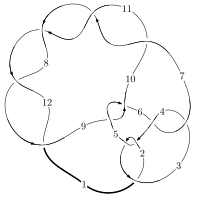
\includegraphics[width=112pt]{../../../GIT/diagram.site/Diagrams/png/2204_12n_0115.png}\\
\ \ \ A knot diagram\footnotemark}&
\allowdisplaybreaks
\textbf{Linearized knot diagam} \\
\cline{2-2}
 &
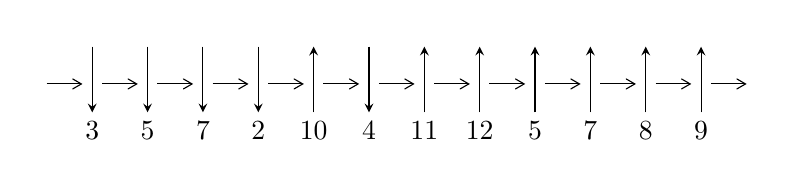
\begin{tikzpicture}[x=20pt, y=17pt]
	% nodes
	\node (C0) at (0, 0) {};
	\node (C1) at (1, 0) {};
	\node (C1U) at (1, +1) {};
	\node (C1D) at (1, -1) {3};

	\node (C2) at (2, 0) {};
	\node (C2U) at (2, +1) {};
	\node (C2D) at (2, -1) {5};

	\node (C3) at (3, 0) {};
	\node (C3U) at (3, +1) {};
	\node (C3D) at (3, -1) {7};

	\node (C4) at (4, 0) {};
	\node (C4U) at (4, +1) {};
	\node (C4D) at (4, -1) {2};

	\node (C5) at (5, 0) {};
	\node (C5U) at (5, +1) {};
	\node (C5D) at (5, -1) {10};

	\node (C6) at (6, 0) {};
	\node (C6U) at (6, +1) {};
	\node (C6D) at (6, -1) {4};

	\node (C7) at (7, 0) {};
	\node (C7U) at (7, +1) {};
	\node (C7D) at (7, -1) {11};

	\node (C8) at (8, 0) {};
	\node (C8U) at (8, +1) {};
	\node (C8D) at (8, -1) {12};

	\node (C9) at (9, 0) {};
	\node (C9U) at (9, +1) {};
	\node (C9D) at (9, -1) {5};

	\node (C10) at (10, 0) {};
	\node (C10U) at (10, +1) {};
	\node (C10D) at (10, -1) {7};

	\node (C11) at (11, 0) {};
	\node (C11U) at (11, +1) {};
	\node (C11D) at (11, -1) {8};

	\node (C12) at (12, 0) {};
	\node (C12U) at (12, +1) {};
	\node (C12D) at (12, -1) {9};
	\node (C13) at (13, 0) {};

	% arrows
	\draw[->,>={angle 60}]
	(C0) edge (C1) (C1) edge (C2) (C2) edge (C3) (C3) edge (C4) (C4) edge (C5) (C5) edge (C6) (C6) edge (C7) (C7) edge (C8) (C8) edge (C9) (C9) edge (C10) (C10) edge (C11) (C11) edge (C12) (C12) edge (C13) ;	\draw[->,>=stealth]
	(C1U) edge (C1D) (C2U) edge (C2D) (C3U) edge (C3D) (C4U) edge (C4D) (C5D) edge (C5U) (C6U) edge (C6D) (C7D) edge (C7U) (C8D) edge (C8U) (C9D) edge (C9U) (C10D) edge (C10U) (C11D) edge (C11U) (C12D) edge (C12U) ;
	\end{tikzpicture} \\
\hhline{~~} \\& 
\textbf{Solving Sequence} \\ \cline{2-2} 
 &
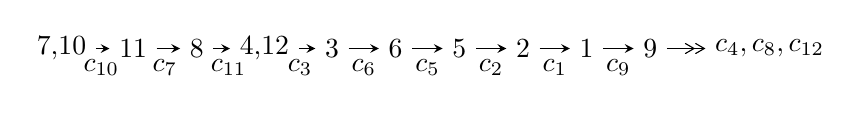
\begin{tikzpicture}[x=23pt, y=7pt]
	% node
	\node (A0) at (-1/8, 0) {7,10};
	\node (A1) at (1, 0) {11};
	\node (A2) at (2, 0) {8};
	\node (A3) at (49/16, 0) {4,12};
	\node (A4) at (33/8, 0) {3};
	\node (A5) at (41/8, 0) {6};
	\node (A6) at (49/8, 0) {5};
	\node (A7) at (57/8, 0) {2};
	\node (A8) at (65/8, 0) {1};
	\node (A9) at (73/8, 0) {9};
	\node (C1) at (1/2, -1) {$c_{10}$};
	\node (C2) at (3/2, -1) {$c_{7}$};
	\node (C3) at (5/2, -1) {$c_{11}$};
	\node (C4) at (29/8, -1) {$c_{3}$};
	\node (C5) at (37/8, -1) {$c_{6}$};
	\node (C6) at (45/8, -1) {$c_{5}$};
	\node (C7) at (53/8, -1) {$c_{2}$};
	\node (C8) at (61/8, -1) {$c_{1}$};
	\node (C9) at (69/8, -1) {$c_{9}$};
	\node (A10) at (11, 0) {$c_{4},c_{8},c_{12}$};

	% edge
	\draw[->,>=stealth]	
	(A0) edge (A1) (A1) edge (A2) (A2) edge (A3) (A3) edge (A4) (A4) edge (A5) (A5) edge (A6) (A6) edge (A7) (A7) edge (A8) (A8) edge (A9) ;
	\draw[->>,>={angle 60}]	
	(A9) edge (A10);
\end{tikzpicture} \\ 

\end{tabular} \\

\footnotetext{
The image of knot diagram is generated by the software ``\textbf{Draw programme}" developed by Andrew Bartholomew(\url{http://www.layer8.co.uk/maths/draw/index.htm\#Running-draw}), where we modified some parts for our purpose(\url{https://github.com/CATsTAILs/LinksPainter}).
}\phantom \\ \newline 
\centering \textbf{Ideals for irreducible components\footnotemark of $X_{\text{par}}$} 
 
\begin{align*}
I^u_{1}&=\langle 
152 u^{13}-2309 u^{12}+\cdots+4348 b+7399,\;-4859 u^{13}+22201 u^{12}+\cdots+4348 a-33463,\\
\phantom{I^u_{1}}&\phantom{= \langle  }u^{14}-5 u^{13}+5 u^{12}+10 u^{11}-13 u^{10}-15 u^9-5 u^8+77 u^7-45 u^6-64 u^5+60 u^4+21 u^3-41 u^2+14 u-1\rangle \\
I^u_{2}&=\langle 
2 a^2 u- a^2+a u+b- a+2 u,\;a^3- a^2 u- a^2+2 a u+4 a-2 u-3,\;u^2+u-1\rangle \\
I^u_{3}&=\langle 
u^2+b- u-2,\;a,\;u^3- u^2-2 u+1\rangle \\
\\
\end{align*}
\raggedright * 3 irreducible components of $\dim_{\mathbb{C}}=0$, with total 23 representations.\\
\footnotetext{All coefficients of polynomials are rational numbers. But the coefficients are sometimes approximated in decimal forms when there is not enough margin.}
\newpage
\renewcommand{\arraystretch}{1}
\centering \section*{I. $I^u_{1}= \langle 152 u^{13}-2309 u^{12}+\cdots+4348 b+7399,\;-4859 u^{13}+22201 u^{12}+\cdots+4348 a-33463,\;u^{14}-5 u^{13}+\cdots+14 u-1 \rangle$}
\flushleft \textbf{(i) Arc colorings}\\
\begin{tabular}{m{7pt} m{180pt} m{7pt} m{180pt} }
\flushright $a_{7}=$&$\begin{pmatrix}0\\u\end{pmatrix}$ \\
\flushright $a_{10}=$&$\begin{pmatrix}1\\0\end{pmatrix}$ \\
\flushright $a_{11}=$&$\begin{pmatrix}1\\- u^2\end{pmatrix}$ \\
\flushright $a_{8}=$&$\begin{pmatrix}u\\- u^3+u\end{pmatrix}$ \\
\flushright $a_{4}=$&$\begin{pmatrix}1.11753 u^{13}-5.10603 u^{12}+\cdots-32.0340 u+7.69618\\-0.0349586 u^{13}+0.531049 u^{12}+\cdots+9.42157 u-1.70170\end{pmatrix}$ \\
\flushright $a_{12}=$&$\begin{pmatrix}- u^2+1\\u^4-2 u^2\end{pmatrix}$ \\
\flushright $a_{3}=$&$\begin{pmatrix}1.11753 u^{13}-5.10603 u^{12}+\cdots-32.0340 u+7.69618\\-0.393514 u^{13}+2.11431 u^{12}+\cdots+15.0465 u-2.18330\end{pmatrix}$ \\
\flushright $a_{6}=$&$\begin{pmatrix}0.332567 u^{13}-1.32498 u^{12}+\cdots-10.1125 u+3.24448\\-0.299908 u^{13}+1.56900 u^{12}+\cdots+9.10350 u-1.05934\end{pmatrix}$ \\
\flushright $a_{5}=$&$\begin{pmatrix}0.632475 u^{13}-2.89397 u^{12}+\cdots-19.2160 u+4.30382\\-0.299908 u^{13}+1.56900 u^{12}+\cdots+9.10350 u-1.05934\end{pmatrix}$ \\
\flushright $a_{2}=$&$\begin{pmatrix}0.632475 u^{13}-2.89397 u^{12}+\cdots-19.2160 u+4.30382\\0.00666973 u^{13}+0.252300 u^{12}+\cdots+7.25345 u-1.30198\end{pmatrix}$ \\
\flushright $a_{1}=$&$\begin{pmatrix}- u^4+3 u^2-1\\u^6-4 u^4+3 u^2\end{pmatrix}$ \\
\flushright $a_{9}=$&$\begin{pmatrix}- u^3+2 u\\u^5-3 u^3+u\end{pmatrix}$\\&\end{tabular}
\flushleft \textbf{(ii) Obstruction class $= -1$}\\~\\
\flushleft \textbf{(iii) Cusp Shapes $= -\frac{11021}{2174} u^{13}+\frac{53061}{2174} u^{12}+\cdots+\frac{369277}{2174} u-\frac{54785}{2174}$}\\~\\
\newpage\renewcommand{\arraystretch}{1}
\flushleft \textbf{(iv) u-Polynomials at the component}\newline \\
\begin{tabular}{m{50pt}|m{274pt}}
Crossings & \hspace{64pt}u-Polynomials at each crossing \\
\hline $$\begin{aligned}c_{1}\end{aligned}$$&$\begin{aligned}
&u^{14}+18 u^{13}+\cdots+1086 u+1
\end{aligned}$\\
\hline $$\begin{aligned}c_{2},c_{4}\end{aligned}$$&$\begin{aligned}
&u^{14}-6 u^{13}+\cdots-34 u-1
\end{aligned}$\\
\hline $$\begin{aligned}c_{3},c_{6}\end{aligned}$$&$\begin{aligned}
&u^{14}-3 u^{13}+\cdots-28 u+8
\end{aligned}$\\
\hline $$\begin{aligned}c_{5},c_{9}\end{aligned}$$&$\begin{aligned}
&u^{14}+2 u^{13}+\cdots+352 u+64
\end{aligned}$\\
\hline $$\begin{aligned}c_{7},c_{8},c_{10}\\c_{11},c_{12}\end{aligned}$$&$\begin{aligned}
&u^{14}-5 u^{13}+\cdots+14 u-1
\end{aligned}$\\
\hline
\end{tabular}\\~\\
\newpage\renewcommand{\arraystretch}{1}
\flushleft \textbf{(v) Riley Polynomials at the component}\newline \\
\begin{tabular}{m{50pt}|m{274pt}}
Crossings & \hspace{64pt}Riley Polynomials at each crossing \\
\hline $$\begin{aligned}c_{1}\end{aligned}$$&$\begin{aligned}
&y^{14}-38 y^{13}+\cdots-1163634 y+1
\end{aligned}$\\
\hline $$\begin{aligned}c_{2},c_{4}\end{aligned}$$&$\begin{aligned}
&y^{14}-18 y^{13}+\cdots-1086 y+1
\end{aligned}$\\
\hline $$\begin{aligned}c_{3},c_{6}\end{aligned}$$&$\begin{aligned}
&y^{14}-15 y^{13}+\cdots-2512 y+64
\end{aligned}$\\
\hline $$\begin{aligned}c_{5},c_{9}\end{aligned}$$&$\begin{aligned}
&y^{14}+30 y^{13}+\cdots-87040 y+4096
\end{aligned}$\\
\hline $$\begin{aligned}c_{7},c_{8},c_{10}\\c_{11},c_{12}\end{aligned}$$&$\begin{aligned}
&y^{14}-15 y^{13}+\cdots-114 y+1
\end{aligned}$\\
\hline
\end{tabular}\\~\\
\newpage\flushleft \textbf{(vi) Complex Volumes and Cusp Shapes}
$$\begin{array}{c|c|c}  
\text{Solutions to }I^u_{1}& \I (\text{vol} + \sqrt{-1}CS) & \text{Cusp shape}\\
 \hline 
\begin{aligned}
u &= -0.847247 + 0.340274 I \\
a &= -1.07919 + 1.10825 I \\
b &= -0.214655 + 0.076845 I\end{aligned}
 & \phantom{-}4.35404 + 2.18891 I & \phantom{-}7.66563 + 1.41199 I \\ \hline\begin{aligned}
u &= -0.847247 - 0.340274 I \\
a &= -1.07919 - 1.10825 I \\
b &= -0.214655 - 0.076845 I\end{aligned}
 & \phantom{-}4.35404 - 2.18891 I & \phantom{-}7.66563 - 1.41199 I \\ \hline\begin{aligned}
u &= \phantom{-}0.683451 + 0.439394 I \\
a &= -0.372092 - 1.119180 I \\
b &= -0.54173 - 1.61181 I\end{aligned}
 & -1.117970 + 0.457834 I & \phantom{-}6.03602 - 2.75865 I \\ \hline\begin{aligned}
u &= \phantom{-}0.683451 - 0.439394 I \\
a &= -0.372092 + 1.119180 I \\
b &= -0.54173 + 1.61181 I\end{aligned}
 & -1.117970 - 0.457834 I & \phantom{-}6.03602 + 2.75865 I \\ \hline\begin{aligned}
u &= \phantom{-}1.293890 + 0.440522 I \\
a &= \phantom{-}0.947194 - 0.804395 I \\
b &= -0.03997 - 1.45852 I\end{aligned}
 & \phantom{-}1.31890 + 3.26489 I & \phantom{-}6.50646 - 2.86357 I \\ \hline\begin{aligned}
u &= \phantom{-}1.293890 - 0.440522 I \\
a &= \phantom{-}0.947194 + 0.804395 I \\
b &= -0.03997 + 1.45852 I\end{aligned}
 & \phantom{-}1.31890 - 3.26489 I & \phantom{-}6.50646 + 2.86357 I \\ \hline\begin{aligned}
u &= -0.79945 + 1.23640 I \\
a &= \phantom{-}0.51219 + 1.76331 I \\
b &= -0.10570 + 1.90296 I\end{aligned}
 & -13.41460 - 4.06288 I & \phantom{-}3.37939 + 1.99626 I \\ \hline\begin{aligned}
u &= -0.79945 - 1.23640 I \\
a &= \phantom{-}0.51219 - 1.76331 I \\
b &= -0.10570 - 1.90296 I\end{aligned}
 & -13.41460 + 4.06288 I & \phantom{-}3.37939 - 1.99626 I \\ \hline\begin{aligned}
u &= \phantom{-}0.485579\phantom{ +0.000000I} \\
a &= -0.359180\phantom{ +0.000000I} \\
b &= \phantom{-}0.426392\phantom{ +0.000000I}\end{aligned}
 & \phantom{-}0.739738\phantom{ +0.000000I} & \phantom{-}13.5200\phantom{ +0.000000I} \\ \hline\begin{aligned}
u &= -1.59630\phantom{ +0.000000I} \\
a &= \phantom{-}0.385525\phantom{ +0.000000I} \\
b &= -1.79529\phantom{ +0.000000I}\end{aligned}
 & \phantom{-}7.97868\phantom{ +0.000000I} & \phantom{-}20.7070\phantom{ +0.000000I}\\
 \hline 
 \end{array}$$\newpage$$\begin{array}{c|c|c}  
\text{Solutions to }I^u_{1}& \I (\text{vol} + \sqrt{-1}CS) & \text{Cusp shape}\\
 \hline 
\begin{aligned}
u &= \phantom{-}1.74684 + 0.37580 I \\
a &= -0.709908 + 0.913168 I \\
b &= \phantom{-}0.34316 + 1.93469 I\end{aligned}
 & -5.06340 + 10.16720 I & \phantom{-}5.53186 - 3.95031 I \\ \hline\begin{aligned}
u &= \phantom{-}1.74684 - 0.37580 I \\
a &= -0.709908 - 0.913168 I \\
b &= \phantom{-}0.34316 - 1.93469 I\end{aligned}
 & -5.06340 - 10.16720 I & \phantom{-}5.53186 + 3.95031 I \\ \hline\begin{aligned}
u &= \phantom{-}1.85818\phantom{ +0.000000I} \\
a &= \phantom{-}0.512193\phantom{ +0.000000I} \\
b &= \phantom{-}0.340829\phantom{ +0.000000I}\end{aligned}
 & \phantom{-}15.4110\phantom{ +0.000000I} & \phantom{-}1.86040\phantom{ +0.000000I} \\ \hline\begin{aligned}
u &= \phantom{-}0.0975686\phantom{ +0.000000I} \\
a &= \phantom{-}4.86506\phantom{ +0.000000I} \\
b &= -0.854160\phantom{ +0.000000I}\end{aligned}
 & -1.21825\phantom{ +0.000000I} & -10.3270\phantom{ +0.000000I}\\
 \hline 
 \end{array}$$\newpage\newpage\renewcommand{\arraystretch}{1}
\centering \section*{II. $I^u_{2}= \langle 2 a^2 u- a^2+a u+b- a+2 u,\;a^3- a^2 u- a^2+2 a u+4 a-2 u-3,\;u^2+u-1 \rangle$}
\flushleft \textbf{(i) Arc colorings}\\
\begin{tabular}{m{7pt} m{180pt} m{7pt} m{180pt} }
\flushright $a_{7}=$&$\begin{pmatrix}0\\u\end{pmatrix}$ \\
\flushright $a_{10}=$&$\begin{pmatrix}1\\0\end{pmatrix}$ \\
\flushright $a_{11}=$&$\begin{pmatrix}1\\u-1\end{pmatrix}$ \\
\flushright $a_{8}=$&$\begin{pmatrix}u\\- u+1\end{pmatrix}$ \\
\flushright $a_{4}=$&$\begin{pmatrix}a\\-2 a^2 u+a^2- a u+a-2 u\end{pmatrix}$ \\
\flushright $a_{12}=$&$\begin{pmatrix}u\\- u\end{pmatrix}$ \\
\flushright $a_{3}=$&$\begin{pmatrix}a\\-2 a^2 u+a^2-2 u\end{pmatrix}$ \\
\flushright $a_{6}=$&$\begin{pmatrix}a^2 u\\0\end{pmatrix}$ \\
\flushright $a_{5}=$&$\begin{pmatrix}a^2 u\\0\end{pmatrix}$ \\
\flushright $a_{2}=$&$\begin{pmatrix}a^2 u\\-2 a^2 u+a^2-2 u\end{pmatrix}$ \\
\flushright $a_{1}=$&$\begin{pmatrix}0\\- u\end{pmatrix}$ \\
\flushright $a_{9}=$&$\begin{pmatrix}1\\0\end{pmatrix}$\\&\end{tabular}
\flushleft \textbf{(ii) Obstruction class $= 1$}\\~\\
\flushleft \textbf{(iii) Cusp Shapes $= 19 a^2 u-13 a^2+9 a u- a+8 u-9$}\\~\\
\newpage\renewcommand{\arraystretch}{1}
\flushleft \textbf{(iv) u-Polynomials at the component}\newline \\
\begin{tabular}{m{50pt}|m{274pt}}
Crossings & \hspace{64pt}u-Polynomials at each crossing \\
\hline $$\begin{aligned}c_{1},c_{3}\end{aligned}$$&$\begin{aligned}
&(u^3- u^2+2 u-1)^2
\end{aligned}$\\
\hline $$\begin{aligned}c_{2}\end{aligned}$$&$\begin{aligned}
&(u^3+u^2-1)^2
\end{aligned}$\\
\hline $$\begin{aligned}c_{4}\end{aligned}$$&$\begin{aligned}
&(u^3- u^2+1)^2
\end{aligned}$\\
\hline $$\begin{aligned}c_{5},c_{9}\end{aligned}$$&$\begin{aligned}
&u^6
\end{aligned}$\\
\hline $$\begin{aligned}c_{6}\end{aligned}$$&$\begin{aligned}
&(u^3+u^2+2 u+1)^2
\end{aligned}$\\
\hline $$\begin{aligned}c_{7},c_{8}\end{aligned}$$&$\begin{aligned}
&(u^2- u-1)^3
\end{aligned}$\\
\hline $$\begin{aligned}c_{10},c_{11},c_{12}\end{aligned}$$&$\begin{aligned}
&(u^2+u-1)^3
\end{aligned}$\\
\hline
\end{tabular}\\~\\
\newpage\renewcommand{\arraystretch}{1}
\flushleft \textbf{(v) Riley Polynomials at the component}\newline \\
\begin{tabular}{m{50pt}|m{274pt}}
Crossings & \hspace{64pt}Riley Polynomials at each crossing \\
\hline $$\begin{aligned}c_{1},c_{3},c_{6}\end{aligned}$$&$\begin{aligned}
&(y^3+3 y^2+2 y-1)^2
\end{aligned}$\\
\hline $$\begin{aligned}c_{2},c_{4}\end{aligned}$$&$\begin{aligned}
&(y^3- y^2+2 y-1)^2
\end{aligned}$\\
\hline $$\begin{aligned}c_{5},c_{9}\end{aligned}$$&$\begin{aligned}
&y^6
\end{aligned}$\\
\hline $$\begin{aligned}c_{7},c_{8},c_{10}\\c_{11},c_{12}\end{aligned}$$&$\begin{aligned}
&(y^2-3 y+1)^3
\end{aligned}$\\
\hline
\end{tabular}\\~\\
\newpage\flushleft \textbf{(vi) Complex Volumes and Cusp Shapes}
$$\begin{array}{c|c|c}  
\text{Solutions to }I^u_{2}& \I (\text{vol} + \sqrt{-1}CS) & \text{Cusp shape}\\
 \hline 
\begin{aligned}
u &= \phantom{-}0.618034\phantom{ +0.000000I} \\
a &= \phantom{-}0.922021\phantom{ +0.000000I} \\
b &= -1.08457\phantom{ +0.000000I}\end{aligned}
 & -0.126494\phantom{ +0.000000I} & -0.918090\phantom{ +0.000000I} \\ \hline\begin{aligned}
u &= \phantom{-}0.618034\phantom{ +0.000000I} \\
a &= \phantom{-}0.34801 + 2.11500 I \\
b &= -0.075747 + 0.460350 I\end{aligned}
 & \phantom{-}4.01109 - 2.82812 I & \phantom{-}3.00413 + 7.79836 I \\ \hline\begin{aligned}
u &= \phantom{-}0.618034\phantom{ +0.000000I} \\
a &= \phantom{-}0.34801 - 2.11500 I \\
b &= -0.075747 - 0.460350 I\end{aligned}
 & \phantom{-}4.01109 + 2.82812 I & \phantom{-}3.00413 - 7.79836 I \\ \hline\begin{aligned}
u &= -1.61803\phantom{ +0.000000I} \\
a &= -0.132927 + 0.807858 I \\
b &= \phantom{-}0.198308 + 1.205210 I\end{aligned}
 & \phantom{-}11.90680 + 2.82812 I & \phantom{-}7.89941 - 3.17745 I \\ \hline\begin{aligned}
u &= -1.61803\phantom{ +0.000000I} \\
a &= -0.132927 - 0.807858 I \\
b &= \phantom{-}0.198308 - 1.205210 I\end{aligned}
 & \phantom{-}11.90680 - 2.82812 I & \phantom{-}7.89941 + 3.17745 I \\ \hline\begin{aligned}
u &= -1.61803\phantom{ +0.000000I} \\
a &= -0.352181\phantom{ +0.000000I} \\
b &= \phantom{-}2.83945\phantom{ +0.000000I}\end{aligned}
 & \phantom{-}7.76919\phantom{ +0.000000I} & -21.8890\phantom{ +0.000000I}\\
 \hline 
 \end{array}$$\newpage\newpage\renewcommand{\arraystretch}{1}
\centering \section*{III. $I^u_{3}= \langle u^2+b- u-2,\;a,\;u^3- u^2-2 u+1 \rangle$}
\flushleft \textbf{(i) Arc colorings}\\
\begin{tabular}{m{7pt} m{180pt} m{7pt} m{180pt} }
\flushright $a_{7}=$&$\begin{pmatrix}0\\u\end{pmatrix}$ \\
\flushright $a_{10}=$&$\begin{pmatrix}1\\0\end{pmatrix}$ \\
\flushright $a_{11}=$&$\begin{pmatrix}1\\- u^2\end{pmatrix}$ \\
\flushright $a_{8}=$&$\begin{pmatrix}u\\- u^2- u+1\end{pmatrix}$ \\
\flushright $a_{4}=$&$\begin{pmatrix}0\\- u^2+u+2\end{pmatrix}$ \\
\flushright $a_{12}=$&$\begin{pmatrix}- u^2+1\\u^2+u-1\end{pmatrix}$ \\
\flushright $a_{3}=$&$\begin{pmatrix}0\\- u^2+u+2\end{pmatrix}$ \\
\flushright $a_{6}=$&$\begin{pmatrix}0\\u\end{pmatrix}$ \\
\flushright $a_{5}=$&$\begin{pmatrix}- u\\u\end{pmatrix}$ \\
\flushright $a_{2}=$&$\begin{pmatrix}u\\- u^2+2\end{pmatrix}$ \\
\flushright $a_{1}=$&$\begin{pmatrix}u\\- u\end{pmatrix}$ \\
\flushright $a_{9}=$&$\begin{pmatrix}- u^2+1\\u^2\end{pmatrix}$\\&\end{tabular}
\flushleft \textbf{(ii) Obstruction class $= 1$}\\~\\
\flushleft \textbf{(iii) Cusp Shapes $= -8 u^2+7 u+30$}\\~\\
\newpage\renewcommand{\arraystretch}{1}
\flushleft \textbf{(iv) u-Polynomials at the component}\newline \\
\begin{tabular}{m{50pt}|m{274pt}}
Crossings & \hspace{64pt}u-Polynomials at each crossing \\
\hline $$\begin{aligned}c_{1},c_{2}\end{aligned}$$&$\begin{aligned}
&(u-1)^3
\end{aligned}$\\
\hline $$\begin{aligned}c_{3},c_{6}\end{aligned}$$&$\begin{aligned}
&u^3
\end{aligned}$\\
\hline $$\begin{aligned}c_{4}\end{aligned}$$&$\begin{aligned}
&(u+1)^3
\end{aligned}$\\
\hline $$\begin{aligned}c_{5},c_{7},c_{8}\end{aligned}$$&$\begin{aligned}
&u^3+u^2-2 u-1
\end{aligned}$\\
\hline $$\begin{aligned}c_{9},c_{10},c_{11}\\c_{12}\end{aligned}$$&$\begin{aligned}
&u^3- u^2-2 u+1
\end{aligned}$\\
\hline
\end{tabular}\\~\\
\newpage\renewcommand{\arraystretch}{1}
\flushleft \textbf{(v) Riley Polynomials at the component}\newline \\
\begin{tabular}{m{50pt}|m{274pt}}
Crossings & \hspace{64pt}Riley Polynomials at each crossing \\
\hline $$\begin{aligned}c_{1},c_{2},c_{4}\end{aligned}$$&$\begin{aligned}
&(y-1)^3
\end{aligned}$\\
\hline $$\begin{aligned}c_{3},c_{6}\end{aligned}$$&$\begin{aligned}
&y^3
\end{aligned}$\\
\hline $$\begin{aligned}c_{5},c_{7},c_{8}\\c_{9},c_{10},c_{11}\\c_{12}\end{aligned}$$&$\begin{aligned}
&y^3-5 y^2+6 y-1
\end{aligned}$\\
\hline
\end{tabular}\\~\\
\newpage\flushleft \textbf{(vi) Complex Volumes and Cusp Shapes}
$$\begin{array}{c|c|c}  
\text{Solutions to }I^u_{3}& \I (\text{vol} + \sqrt{-1}CS) & \text{Cusp shape}\\
 \hline 
\begin{aligned}
u &= -1.24698\phantom{ +0.000000I} \\
a &= \phantom{-0.000000 } 0 \\
b &= -0.801938\phantom{ +0.000000I}\end{aligned}
 & \phantom{-}4.69981\phantom{ +0.000000I} & \phantom{-}8.83150\phantom{ +0.000000I} \\ \hline\begin{aligned}
u &= \phantom{-}0.445042\phantom{ +0.000000I} \\
a &= \phantom{-0.000000 } 0 \\
b &= \phantom{-}2.24698\phantom{ +0.000000I}\end{aligned}
 & -0.939962\phantom{ +0.000000I} & \phantom{-}31.5310\phantom{ +0.000000I} \\ \hline\begin{aligned}
u &= \phantom{-}1.80194\phantom{ +0.000000I} \\
a &= \phantom{-0.000000 } 0 \\
b &= \phantom{-}0.554958\phantom{ +0.000000I}\end{aligned}
 & \phantom{-}15.9794\phantom{ +0.000000I} & \phantom{-}16.6380\phantom{ +0.000000I}\\
 \hline 
 \end{array}$$\newpage
\newpage\renewcommand{\arraystretch}{1}
\centering \section*{ IV. u-Polynomials}
\begin{tabular}{m{50pt}|m{274pt}}
Crossings & \hspace{64pt}u-Polynomials at each crossing \\
\hline $$\begin{aligned}c_{1}\end{aligned}$$&$\begin{aligned}
&((u-1)^3)(u^3- u^2+2 u-1)^2(u^{14}+18 u^{13}+\cdots+1086 u+1)
\end{aligned}$\\
\hline $$\begin{aligned}c_{2}\end{aligned}$$&$\begin{aligned}
&((u-1)^3)(u^3+u^2-1)^2(u^{14}-6 u^{13}+\cdots-34 u-1)
\end{aligned}$\\
\hline $$\begin{aligned}c_{3}\end{aligned}$$&$\begin{aligned}
&u^3(u^3- u^2+2 u-1)^2(u^{14}-3 u^{13}+\cdots-28 u+8)
\end{aligned}$\\
\hline $$\begin{aligned}c_{4}\end{aligned}$$&$\begin{aligned}
&((u+1)^3)(u^3- u^2+1)^2(u^{14}-6 u^{13}+\cdots-34 u-1)
\end{aligned}$\\
\hline $$\begin{aligned}c_{5}\end{aligned}$$&$\begin{aligned}
&u^6(u^3+u^2-2 u-1)(u^{14}+2 u^{13}+\cdots+352 u+64)
\end{aligned}$\\
\hline $$\begin{aligned}c_{6}\end{aligned}$$&$\begin{aligned}
&u^3(u^3+u^2+2 u+1)^2(u^{14}-3 u^{13}+\cdots-28 u+8)
\end{aligned}$\\
\hline $$\begin{aligned}c_{7},c_{8}\end{aligned}$$&$\begin{aligned}
&((u^2- u-1)^3)(u^3+u^2-2 u-1)(u^{14}-5 u^{13}+\cdots+14 u-1)
\end{aligned}$\\
\hline $$\begin{aligned}c_{9}\end{aligned}$$&$\begin{aligned}
&u^6(u^3- u^2-2 u+1)(u^{14}+2 u^{13}+\cdots+352 u+64)
\end{aligned}$\\
\hline $$\begin{aligned}c_{10},c_{11},c_{12}\end{aligned}$$&$\begin{aligned}
&((u^2+u-1)^3)(u^3- u^2-2 u+1)(u^{14}-5 u^{13}+\cdots+14 u-1)
\end{aligned}$\\
\hline
\end{tabular}\newpage\renewcommand{\arraystretch}{1}
\centering \section*{ V. Riley Polynomials}
\begin{tabular}{m{50pt}|m{274pt}}
Crossings & \hspace{64pt}Riley Polynomials at each crossing \\
\hline $$\begin{aligned}c_{1}\end{aligned}$$&$\begin{aligned}
&((y-1)^3)(y^3+3 y^2+2 y-1)^2(y^{14}-38 y^{13}+\cdots-1163634 y+1)
\end{aligned}$\\
\hline $$\begin{aligned}c_{2},c_{4}\end{aligned}$$&$\begin{aligned}
&((y-1)^3)(y^3- y^2+2 y-1)^2(y^{14}-18 y^{13}+\cdots-1086 y+1)
\end{aligned}$\\
\hline $$\begin{aligned}c_{3},c_{6}\end{aligned}$$&$\begin{aligned}
&y^3(y^3+3 y^2+2 y-1)^2(y^{14}-15 y^{13}+\cdots-2512 y+64)
\end{aligned}$\\
\hline $$\begin{aligned}c_{5},c_{9}\end{aligned}$$&$\begin{aligned}
&y^6(y^3-5 y^2+6 y-1)(y^{14}+30 y^{13}+\cdots-87040 y+4096)
\end{aligned}$\\
\hline $$\begin{aligned}c_{7},c_{8},c_{10}\\c_{11},c_{12}\end{aligned}$$&$\begin{aligned}
&((y^2-3 y+1)^3)(y^3-5 y^2+6 y-1)(y^{14}-15 y^{13}+\cdots-114 y+1)
\end{aligned}$\\
\hline
\end{tabular}
\vskip 2pc
\end{document}